% Artigo WiP (Work in Progress) para o ICIT 2027, no modelo de conferência do IEEE.
% Limite: 4 páginas, já contando figuras e referências. Submissão: 3/11/2026 (prazo final).
% A bibliografia vem de ../referencial/references.bib (não duplicar).
\documentclass[conference]{IEEEtran}
\IEEEoverridecommandlockouts

\usepackage[T1]{fontenc}
\usepackage[utf8]{inputenc}
\usepackage{cite}
\usepackage{amsmath,amssymb,amsfonts}
\usepackage{graphicx}
\usepackage{booktabs}
\usepackage{array}
\usepackage{url}
\usepackage{tikz}
\usetikzlibrary{positioning,fit,arrows.meta}

\begin{document}

\title{Toward a Capability Specification for\\
Kubernetes-Based Supervision of Process Plants}

\author{
\IEEEauthorblockN{Matheus Corteletti Delfino}
\IEEEauthorblockA{\textit{Control and Automation Engineering} \\
\textit{Instituto Federal do Espírito Santo (Ifes)}\\
Serra, ES, Brazil \\
matheus.corteletti.del@gmail.com}
\and
\IEEEauthorblockN{Rafael Emerick Zape de Oliveira}
\IEEEauthorblockA{\textit{Control and Automation Engineering} \\
\textit{Instituto Federal do Espírito Santo (Ifes)}\\
Serra, ES, Brazil \\
rafael.emerick@ifes.edu.br}
}

\maketitle

\begin{abstract}
Kubernetes keeps software systems close to a declared desired state, and recent work uses it to run industrial control software. This work in progress asks a different question: what must an implementation demonstrate before one can say that a process plant is under Kubernetes-based supervision? We propose a specification organized in four verifiable capabilities: observing the operation against a declared policy, evaluating and executing operating changes, managing devices and versions, and integrating equipment through OPC~UA. We then report a first open implementation that demonstrates the first capability on a simulation of the Tennessee Eastman Process. The simulated plant reproduces the published operating costs of the base case (170.63 against 170.61~\$/h) and of the Mode~1 optimum (114.32 against 114.31~\$/h). With the plant running about ten times faster than real time, a Kubernetes controller evaluated it against the declared policy every 30~s and flagged a feed loss 1.15~h of process time after it occurred. In another run, cost fell 37\% in 30~h while the plant drifted toward shutdown, and only a declared level limit flagged it, 2~h before the shutdown. We describe the plan for the remaining capabilities and a validation protocol open to other implementations.
\end{abstract}

\begin{IEEEkeywords}
Kubernetes, process supervision, operating policy, OPC UA, Tennessee Eastman Process, digital twin, reference architecture
\end{IEEEkeywords}

\section{Introduction}

Process plants are operated in layers \cite{Skogestad2004}. Controllers keep variables such as levels and pressures at their setpoints, and a supervisory layer chooses those setpoints and checks whether the plant does what was decided. In the enterprise-control hierarchy of IEC~62264 \cite{IEC62264}, this supervision sits between the control systems and the business systems. In practice, the engineers who know how to improve a plant (chemical, mechanical and control engineers) often work on data exported from the historian and analyzed offline.

Software engineering faces a similar problem in distributed systems. Kubernetes is a container orchestration platform with a declarative interface: the user declares the desired state as resources, and controllers continuously bring the observed state toward it \cite{Burns2016}. New resource types and controllers can be added without changing the platform. This suggests using Kubernetes as the supervisory layer of a plant: the operating policy becomes a declared resource, and a controller reconciles the plant against it.

Using Kubernetes is not enough to say that a plant is supervised. A company that claims to follow an information security standard must show that certain processes exist, regardless of the tools it uses. In the same spirit, we ask what an implementation must demonstrate before one can say that a plant is under Kubernetes-based supervision. This paper contributes:
\begin{itemize}
\item a specification organized in four verifiable capabilities, each with what an implementation must demonstrate (Section~\ref{sec:spec});
\item a first open implementation that demonstrates the first capability on the Tennessee Eastman Process (TEP) \cite{DOWNS1993}, with results (Sections~\ref{sec:impl} and~\ref{sec:results});
\item a plan for the remaining capabilities and a validation protocol open to other implementations (Section~\ref{sec:ongoing}).
\end{itemize}
The specification is a proposal, not a standard. We submit it at this stage to receive criticism before the remaining capabilities are built.

\section{Related Work}

Kubernetes has reached industrial automation mainly as infrastructure for control software. Johansson et~al.\ use it to recover failed controllers with high availability \cite{Johansson2022}, Mellado and Núñez run a programmable logic controller in containers \cite{Mellado2022}, and Koziolek and Burger use a purpose-built Kubernetes operator to update virtual controllers without halting production \cite{Koziolek2022}. In these cases, Kubernetes manages the software that controls the process, not the decisions about how the process should operate. Cloud-native practice in general is surveyed in \cite{Shuiguang2023}.

The supervisory functions themselves have long roots. Autonomic computing organizes self-management as monitoring, analysis, planning and execution over shared knowledge \cite{Kephart2003}. Reference governors change setpoints so that constraints are respected during transitions \cite{Gilbert1995,Garone2017}, and digital twins support prediction and control \cite{Kritzinger2018,Zhao2023}. OPC~UA is the standard way for equipment to expose data and methods \cite{IEC62541_1}. The works above do not define what a Kubernetes-based supervisory layer must demonstrate, which is the gap this paper addresses.

\section{Capability Specification}
\label{sec:spec}

Table~\ref{tab:caps} lists the four capabilities. Kubernetes is the base that coordinates them; the specification gives them an industrial meaning and states the conditions for considering them met. An implementation may demonstrate only some capabilities, and it reports which ones and with what evidence.

\begin{table*}[t]
\caption{Capabilities of Kubernetes-based plant supervision}
\label{tab:caps}
\centering
\footnotesize
\begin{tabular}{@{}>{\raggedright\arraybackslash}p{0.17\textwidth}>{\raggedright\arraybackslash}p{0.49\textwidth}>{\raggedright\arraybackslash}p{0.27\textwidth}@{}}
\toprule
Capability & What an implementation must demonstrate & Status in this work \\
\midrule
C1 Observe the operation & The supervisor receives enough up-to-date data to compare the plant with the declared policy, and records its verdict as Kubernetes state. & Demonstrated on the simulated TEP (Section~\ref{sec:results}). \\
C2 Evaluate and execute changes & A change in the declaration starts a procedure: prepare a digital twin synchronized with the plant, test the change, evaluate the criteria, authorize or refuse, apply, and verify the plant response, including when the result is inconclusive or a component fails. & Planned. The current supervisor never writes to the plant. \\
C3 Manage devices and versions & Keep an inventory of devices, software and configuration versions and the history of changes, separating the declared state from the state found in the plant. & Planned. \\
C4 Integrate through OPC~UA & Define how equipment exposes data and commands, with identification, permissions and handling of communication failures. & Reading demonstrated; writing, permissions and failures not yet evaluated. \\
\bottomrule
\end{tabular}
\end{table*}

Three design rules apply to all capabilities. First, the supervisor knows the plant only through the declared resources, so that the same supervisor can, in principle, serve another plant; this has not been tested yet. Second, verdicts and decisions are stored in Kubernetes itself, where any client can read them and where they leave a record. Third, control and safety functions stay in the plant controllers: the supervisor is never in the real-time path, and the plant must stay safe if the supervisor fails.

\section{First Implementation}
\label{sec:impl}

The implementation is open source\footnote{\raggedright\url{https://github.com/Green-Cinnamon-Labs}.\\ Start at the \texttt{spec-tennessee-eastman} repository.} and has four components (Fig.~\ref{fig:arch}).

\begin{figure}[t]
\centering
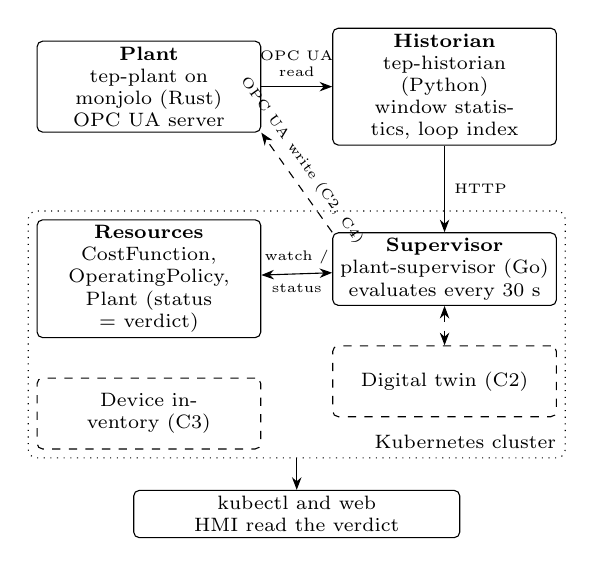
\begin{tikzpicture}[
  >={Stealth[length=1.6mm]},
  box/.style={draw, rounded corners=2pt, align=center, font=\scriptsize,
              minimum height=9mm, text width=27mm, inner sep=2pt},
  plan/.style={box, dashed},
  lbl/.style={font=\tiny, align=center}]
\node[box] (plant) {\textbf{Plant}\\ tep-plant on monjolo (Rust)\\ OPC~UA server};
\node[box, right=9mm of plant] (hist) {\textbf{Historian}\\ tep-historian (Python)\\ window statistics, loop index};
\node[box, below=11mm of hist] (sup) {\textbf{Supervisor}\\ plant-supervisor (Go)\\ evaluates every 30~s};
\node[box, below=11mm of plant] (res) {\textbf{Resources}\\ CostFunction, OperatingPolicy,\\ Plant (status = verdict)};
\node[plan, below=5mm of sup] (twin) {Digital twin (C2)};
\node[plan, below=5mm of res] (inv) {Device inventory (C3)};
\node[draw, dotted, rounded corners=3pt, inner sep=3pt,
      fit=(res)(sup)(twin)(inv),
      label={[font=\scriptsize, anchor=south east]south east:Kubernetes cluster}] (k8s) {};
\node[box, below=4mm of k8s, text width=40mm, minimum height=6mm] (hmi) {kubectl and web HMI read the verdict};
\draw[->] (plant) -- node[lbl, above] {OPC~UA\\read} (hist);
\draw[->] (hist) -- node[lbl, right] {HTTP} (sup);
\draw[<->] (sup) -- node[lbl, above] {watch /}node[lbl, below] {status} (res);
\draw[->, dashed] (sup.north west) -- node[lbl, sloped, above, pos=0.62] {OPC~UA write (C2, C4)} (plant.south east);
\draw[<->, dashed] (sup) -- (twin);
\draw[->] (k8s.south -| hmi.north) ++(0,0) -- (hmi.north);
\end{tikzpicture}
\caption{Architecture of the first implementation. Solid: built and evaluated. Dashed: planned.}
\label{fig:arch}
\end{figure}

\textit{Plant.} The Downs and Vogel model \cite{DOWNS1993} was rewritten in Rust as a plant that runs continuously and publishes its signals over OPC~UA. The generic part (state registry, integrator, actuator and sensor blocks, OPC~UA adapter) was separated into a runtime called \texttt{monjolo}, which knows nothing about the TEP. The plant can run faster than real time.

\textit{Historian.} A Python service collects every signal over OPC~UA, keeps the last 15~minutes, and serves window statistics and a control loop performance index \cite{Bradu2018} over HTTP. Kubernetes never sees raw signals, only these aggregates.

\textit{Supervisor.} A Kubernetes controller written in Go reads three custom resources. \texttt{CostFunction} declares the operating cost as a sum of terms; \texttt{OperatingPolicy} declares the cost budget, production targets, variable limits, control loops to watch, and how many bad evaluations in a row change the verdict; \texttt{Plant} links them to a plant and holds the verdict. Every 30~s, the supervisor queries the historian and writes into the \texttt{Plant} status the conditions \texttt{CostWithinBudget}, \texttt{ConstraintsSatisfied} and \texttt{ControlLoopsHealthy} and a phase, compliant or not. The policy can be edited with \texttt{kubectl} while the supervisor runs, and is re-evaluated immediately.

\textit{Interface.} The verdict is read with \texttt{kubectl} or in a web HMI. The cluster is a single local node.

\section{Preliminary Results}
\label{sec:results}

All times below are process times. The plant was accelerated, but the 30~s evaluation period is wall-clock time, so each evaluation covered more process time than it would in real operation.

\textit{Model check.} Table~\ref{tab:calib} compares the operating cost of the simulated plant with the published values. The Mode~1 value comes from a plant version with integrated cooling water. This checks the steady state of the model, not its dynamics.

\begin{table}[t]
\caption{Operating cost of the simulated plant}
\label{tab:calib}
\centering
\footnotesize
\begin{tabular}{@{}lcc@{}}
\toprule
Operating point & Published (\$/h) & This work (\$/h) \\
\midrule
Base case \cite{DOWNS1993} & 170.61 & 170.63 \\
Mode~1 optimum \cite{Ricker1995} & 114.31 & 114.32 \\
\bottomrule
\end{tabular}
\end{table}

\textit{Normal operation.} The Mode~1 policy was calibrated on a run without disturbance, at about ten times real time: over 41 evaluations, the cost stayed at $166.83 \pm 0.18$~\$/h and all conditions held. The cost budget was set at 170.6~\$/h, the cost of the base case.

\textit{Feed loss.} At about ten times real time (about 5~min of process per evaluation), with the policy fixed, disturbance IDV(6), the loss of feed A, was applied. The product flow left its target 0.98~h after the disturbance, and the cost exceeded the budget at 1.15~h (about 7~min of wall-clock time), when the phase changed to non-compliant: the verdict followed the physical order of events. The loop index alone did not flag the disturbance. A setpoint tracking criterion was added, which required changing the supervisor code, not only the policy; in a repeated run with it, the levels crossed the declared limit at 0.84~h and the loop condition turned false at 1.00~h. A later re-reading of the data showed that the index was computed on an inverted scale, which explains part of this blindness.

\textit{Cost that improves while the plant degrades.} With the three control loops changed from proportional to PI, and no reactor level loop, the plant ran without disturbance at about 56 times real time (about 28~min of process per evaluation). The purge valve closed slowly, inert gas accumulated and the reactor level fell from 71.6\% to 47.8\% in 30~h, until the reactor pressure crossed the 3000~kPa shutdown limit at 32.9~h. Throughout this run, the cost fell, from 165.9 to 105.3~\$/h in 30~h, because less reactant left in the purge; the cost condition held in all 70 evaluations, and the loops stayed healthy. Only the reactor level limit declared in the policy (at least 50\%) noticed, with a non-compliant verdict at 30.9~h, close to the physical loss. Part of this delay comes from the acceleration, but the level had also fallen for about 25~h inside the allowed range: a fixed limit warns when a variable arrives, not when it starts to drift.

\textit{What this shows for C1.} A Kubernetes controller can follow a running simulated plant through a historian, from a policy that the user declares and edits. This was not tested in real time, on a physical plant or on a multi-node cluster. The runs also show the limits of observation: a useful policy must watch inventories and trends, not only cost and loops, and a new type of criterion still requires code. The last run is also the main motivation for C2: when the supervisor only observes, a correct verdict may come too late to act on.

\section{Ongoing Work and Validation Plan}
\label{sec:ongoing}

\textit{C2: changes as progressive rollouts.} We are designing the supervisor to treat a setpoint change as Kubernetes treats a software deployment: applied in steps, verified, and rolled back if a declared condition fails. Before each step, the supervisor synchronizes a digital twin with the plant and simulates the step faster than real time; if the simulation violates the policy, the step is refused and the refusal is recorded. Three strategies will be compared with the same code: applying the change at once, in steps, and in steps tested on the twin. The comparison will measure the area, duration and peak of limit violations, completed and refused changes, and decision latency, also with deliberate errors in the twin parameters.

\textit{Second plant.} The target is a didactic level process at Ifes, where a PID in the plant controller drives a pump and the setpoint is exposed through an OPC server. Its model will first be written in \texttt{monjolo}; experiments on the physical plant depend on access and authorization, which have not been confirmed yet. In this plant, the supervisor will only change setpoints; control and protections stay in the controller.

\textit{C3 and C4.} Devices and their software and configuration versions will be represented as Kubernetes resources, with the declared and the found state side by side. The OPC~UA write path will be specified with identification, permissions and behavior under communication loss.

\textit{Validation by others.} To let other groups build and check their own implementations, we plan to simplify the stack: a Python interface for plant models beside the Rust one, a historian template, and a single-command cluster setup. An implementation will claim the capabilities it meets and pass a set of scenario tests for each. We will also measure the effort to bring a new plant under supervision: code written, and changes needed in the supervisor, with the goal of none.

\section{Open Questions and Conclusion}

We would welcome reviewers' views on three questions. Is a capability specification the right way to define Kubernetes-based supervision, and are these four capabilities the right ones? Why Kubernetes rather than a supervisory sequence in SCADA or in the plant controller? Our answer is the life cycle of an operating change, which becomes declared, versioned, reconciled and recorded, using the same tools as other software systems; we would like to know whether this matters to practitioners. And what evidence would convince plant engineers that such a layer is useful?

In summary, the first capability has been demonstrated on a simulated benchmark, with its limits; the others are a research program, with criteria that any implementation can be checked against.

\bibliographystyle{IEEEtran}
\bibliography{../referencial/references}

\end{document}
